{
  \newmdenv[tikzsetting={draw=black,fill=white,fill opacity=0.7, line width=4pt},backgroundcolor=none,leftmargin=0,rightmargin=0,innertopmargin=4pt,skipbelow=\baselineskip,%
  skipabove=\baselineskip]{TitleBoxConclusion}

  \usebackgroundtemplate{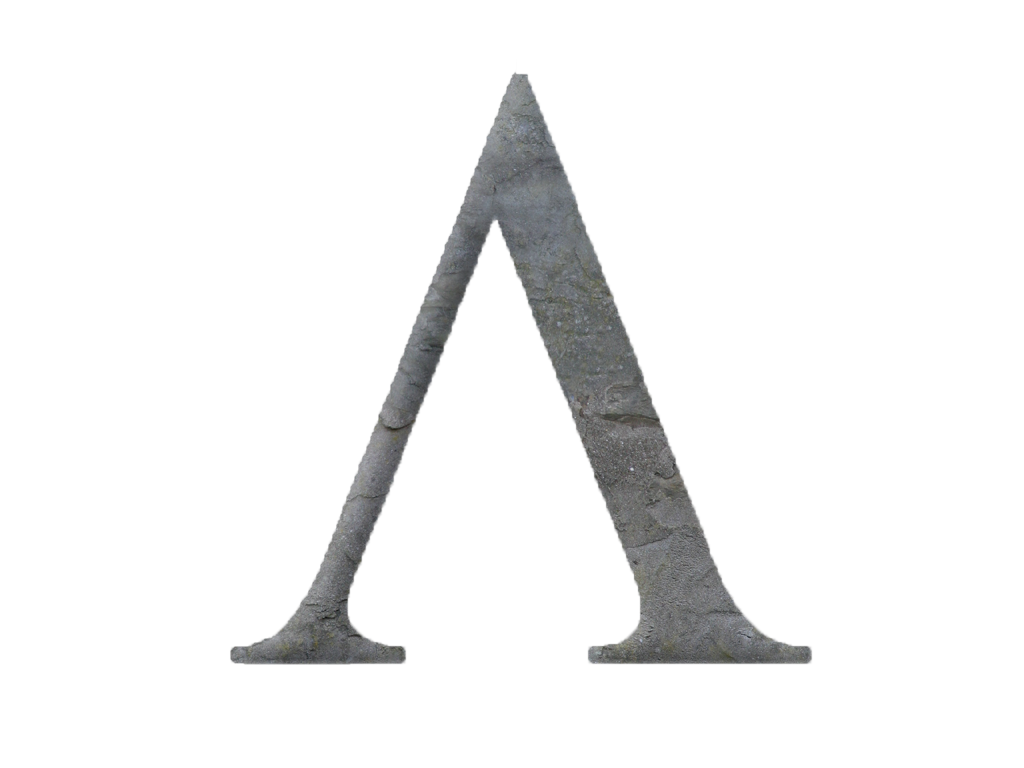
\includegraphics[width=1.0\paperwidth]{image/title-background.png}}

  \begin{frame}[plain] 
  \title{Let's tie it up}
  
  \vspace{3em}

  \begin{TitleBoxConclusion}
    \begin{center}
    {\Large \inserttitle}
    \end{center}
  \end{TitleBoxConclusion}

  \end{frame}
}


\begin{frame}
\frametitle{Django}
\begin{center}
The primary purpose of frameworks like Django is to observe similarities in otherwise disjoint applications \ldots
\end{center}
\vspace{3em}
\begin{center}
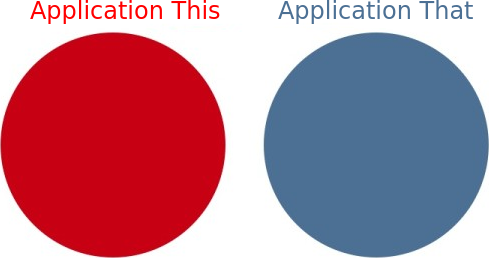
\includegraphics[width=0.4\paperwidth]{image/venn-disjoint.png}
\end{center}
\end{frame}


\begin{frame}
\frametitle{Django}
\begin{center}
\ldots and provide library support for those similarities, while distingushing from differences.
\end{center}
\vspace{3em}
\begin{center}
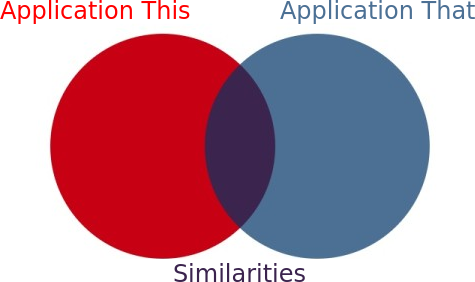
\includegraphics[width=0.4\paperwidth]{image/venn-joined.png}
\end{center}
\end{frame}


\begin{frame}
\frametitle{Django}
\begin{center}
For example, Django \emph{themes} or \emph{templates}
\end{center}
\vspace{3em}
\begin{center}
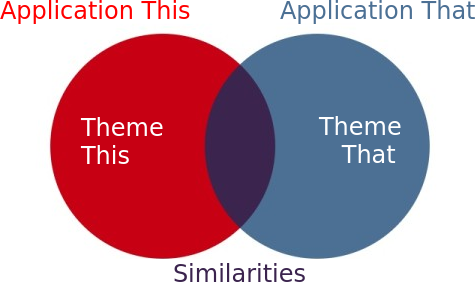
\includegraphics[width=0.4\paperwidth]{image/venn-themes.png}
\end{center}
\end{frame}


\begin{frame}
\frametitle{Bugs}
\begin{block}{Maintenance issues}
Maintenance issues come about when software components leak over these boundaries
\end{block}
\end{frame}


\begin{frame}
\frametitle{Equational Reasoning}
\begin{block}{We have a name for this delineation of concepts}
Equational reasoning
\end{block}
\vspace{3em}
\begin{center}
This is the essence of functional programming!
\end{center}
\end{frame}


\begin{frame}
\frametitle{Tool Support}
OK, so what support do our tools provide us for exploiting this?
\end{frame}


\begin{frame}
\frametitle{Tool Support}
\begin{center}
\huge{0}\normalsize
\end{center}
\vspace{2em}
\begin{center}
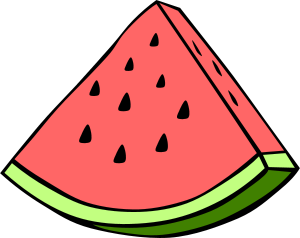
\includegraphics[width=0.3\paperwidth]{image/watermelon.png}
\end{center}
\vspace{1em}
\begin{center}
\tiny{``Is it really such a big deal to rewrite your function to use a loop?''}\normalsize
\end{center}
\end{frame}


\begin{frame}
\frametitle{Tool Support}
\begin{center}
Oh
\end{center}
\vspace{2em}
\begin{center}

\includegraphics[width=0.3\paperwidth]{image/sad-face.jpg}
\end{center}
\vspace{1em}
\begin{center}
Then what about parametricity? Abstraction?
\end{center}
\end{frame}


\begin{frame}
\frametitle{Tool Support}
\begin{center}
\huge{Again, 0}\normalsize
\end{center}
\vspace{2em}
\begin{center}
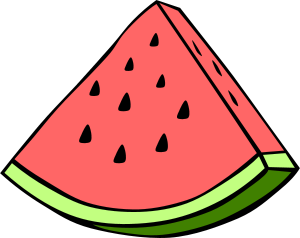
\includegraphics[width=0.3\paperwidth]{image/watermelon.png}
\end{center}
\end{frame}


\begin{frame}
\frametitle{Tool Support}
\begin{block}{More to the point}
There is a \textbf{huge} amount of code that I cannot write without these tools \ldots
\end{block}
\end{frame}


\begin{frame}
\frametitle{Tool Support}
\begin{block}{\ldots and I suspect}
that nobody can, because I never see it
\end{block}
\end{frame}


\begin{frame}
\frametitle{So here's why}
\begin{block}{If you accept}
\begin{itemize}
  \item Equational reasoning
  \item Parametricity
  \item Abstraction
\end{itemize}
\end{block}
\end{frame}


\begin{frame}
\frametitle{So here's why}
\begin{block}{Then you also accept}
\begin{center}
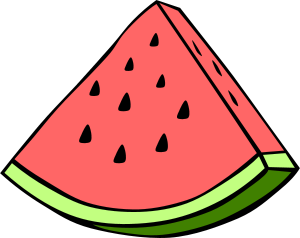
\includegraphics[width=0.3\paperwidth]{image/watermelon.png}
\end{center}
\end{block}
\end{frame}


\begin{frame}
\frametitle{How?}
\begin{block}{How might I learn to exploit these tools?}
\begin{center}
\huge{Diversify}\normalsize
\end{center}
\begin{itemize}
  \item Total programming (Agda, Coq, Idris)
  \item Pure functional programming (Haskell)
\end{itemize}
\end{block}
\end{frame}


\begin{frame}
\frametitle{TL;DR}
\begin{block}{TL;DR}
\begin{center}

\includegraphics[width=0.85\paperwidth]{image/pythonic.png}
\end{center}
\end{block}
\end{frame}
